\documentclass[../book.tex]{subfiles}
\graphicspath{{\subfix{../images/}}}

\begin{document}
\chapter{Conic Sections}
\begin{introduction}[Contents]
\item Parabolas and Applications
\item Circles and Applications
\item Ellipses and Applications
\item Hyperbolas
\item A Note on Rational Functions
\end{introduction}

\noindent In this chapter, we will discuss the four types of conic sections: parabolas, circles, ellipses, hyperbolas.  You are probably familiar with parabolas and circles, which we will review before introducing ellipses and hyperbolas.  Although it may not be apparent initially, conic sections have various applications in many subjects, including astrophysics and optics.  

\begin{remark} 
Of all chapters in Pre-Calculus, many students find conics to be the most difficult.  If you struggle at first, especially with hyperbolas, don't worry!  That's normal.
\end{remark}

\section{Parabolas and Applications}
\subsection{Parabolas as Quadratic Functions}
\noindent Let's start by reviewing parabolas.  Parabolas are arch-shaped curves represented by quadratic equations.  Any equation you've seen in the form $$y(x) = ax^2+bx+c$$
would have a parabolic graph.  The parabola $y=x^2-4x+7$ can be seen to the right.  Up until this point, you have seen three forms for quadratic equations.

\begin{itemize}
    \item Standard Form: $y = ax^2+bx+c$
    \item Vertex Form where $(h,k)$ is the vertex: $y = a(x-h)^2+k $
    \item Factored form where $x=r_1,r_2$ are the roots: $y = a(x-r_1)(x-r_2) $
\end{itemize}

\noindent Now, we introduce a fourth form: $ \frac{1}{a}(y-k) = (x-h)^2$
$(h,k)$ is still the vertex of the parabola.  This form has no name, but is the common form when conics are being discussed.  It is notably similar to vertex form.

\begin{example}
Express $y = x^2-4x+7$ in the form $\frac{1}{a}(y-k)=(x-h)^2$.
\end{example}
\begin{solution}
The method for converting quadratics in standard form to the conic form is clearly similar to that for converting to vertex form.  Start by completing the square.
$$y(x) = x^2 - 4x + 7 $$
Group together a perfect square and factor.
$$y(x) = (x^2 - 4x + 4) + 3 \implies y(x) = (x-2)^2+3 $$
Finally, to convert this to the conic form, simply subtract the constant from both sides.
$$y(x) - 3 = (x-2)^2 $$
There is an implicit $a=1$, but dividing by $1$ on both sides will yield the same equation. $\Box$
\end{solution}
In the context of conics, parabolas have a unique geometric meaning.  All points on a parabola are equidistant between a point called the focus and a line called the directrix.  To find the locations of the focus and the directrix, we first calculate $p = \frac{1}{4a}$.  Then the location of the focus is $(h,k+p)$ and the equation for the directrix is $y = k-p$.  We can rewrite the conic form 

\begin{wrapfigure}{r}{5cm}
    \begin{tikzpicture}[xscale=0.25,yscale=0.25]
        \draw[<->] (-10,0) -- (10,0) node[right] {$x$};
        \draw[<->] (0,-10) -- (0,10) node[above] {$f(x)$};
        \draw[blue,scale=1,variable=\x,domain=-4:8] plot ({\x},{\x*\x/4-\x+2});
        \filldraw[red] (2,2) circle[radius=3pt] node[above] {$(2,2)$};
        \draw[red,scale=1,variable=\x,domain=-10:10] plot ({\x},{0}) node[below left] {$y=0$};
    \end{tikzpicture}
\end{wrapfigure}

\noindent for quadratics in terms of $p$ instead of $a$.
$$4p(y-k) = (x-h)^2 $$

\begin{example}
Find the location of the focus and the equation for the directrix of $y(x) = \frac{1}{4}x^2-x+2$.  Graph the equation, the focus, and the directrix.
\end{example}
\begin{solution}
Start by putting the equation in conic form by first completing the square. \\
Factor out the coefficient of the $x^2$ term.
$$ y = \frac{1}{4}(x^2-4x+8) $$
Extracting the perfect square from the inside we get $$y(x)=\dfrac{1}{4}\big((x^2-4x+4)+4\big) \implies y(x)=\dfrac{1}{4}\big((x-2)^2+4\big)$$$$\implies y(x)=\dfrac{1}{4}(x-2)^2+1.$$
Rearranging this to put it into the proper form, we get $4(y-1) = (x-2)^2$.

We see that $4p = 4 \implies p = 1$ and the vertex of the parabola is $(2,1)$.  Therefore, the focus is at $(2,1+1)\implies(2,2)$ and the directrix is $y = 1-1 \implies y=0$.  The graph can be seen below. $\Box$
\end{solution}

\subsection{Application: Projectile Motion}
\noindent One of the most useful and widely-used applications of parabolas is projectile motion.  When you throw a football or jump in the air, the resulting motion comes in the shape of a parabola.  In such instances, we call the launched object a projectile.  If $g$ is the acceleration due to gravity, $v_0$ is the initial speed, $\theta$ is the launch angle, and $h$ is the initial height of the projectile, then the equation for the projectile's height over time is
$$y(t)=\frac{1}{2}gt^2+v_0t\sin{\theta}+h$$

\begin{remark}
For incoming MSE freshmen, this equation will be vital in your Physics 1 class.
\end{remark}

\begin{example}
The acceleration due to gravity on the surface of the Earth is $g = 10$ m/s$^2$.  Suppose you throw your physics textbook up in the air at $30$ m/s $60^{\circ}$ above the horizontal.  You are $2$ metres tall and launch the textbook right above your head.  Find the equation for the height of the book over time and then graph the equation.
\end{example}
\begin{solution}
Finding the equation for the textbook's height simply requires you to interpret the meaning of each value given in the problem.  NOTE: gravity is in the downward direction, so its value is negative.
\end{solution}
$$ y(t) = \frac{1}{2}gt^2 + v_0t\sin{\theta}+h \implies y(t)=\frac{1}{2}(-10)t^2 + (30)t\sin{(30^\circ)} + (2)= -5t^2 + 30\left(\frac{1}{2}\right)t + 2$$ $$\implies y(t) = -5t^2 + 15t + 2 $$

\begin{wrapfigure}{r}{5cm}
    \begin{tikzpicture}[xscale=0.125,yscale=0.125]
        \draw[<->] (-20,0) -- (20,0) node[right] {$x$};
        \draw[<->] (0,-20) -- (0,20) node[above] {$f(x)$};
        \draw[blue,scale=1,variable=\x,domain=-1.079:4.079] plot ({\x},{-5*\x*\x+15*\x+2});
    \end{tikzpicture}
\end{wrapfigure}

The graph for this equation can be seen below. $\Box$
\subsection{Horizontal Parabolas}
\noindent Up until this point, we've only looked at "vertical" parabolas, or those that pass the vertical line test and have equations in the form:
$$ 4p(y-k) = (x-h)^2 $$
In this section, we will examine "horizontal" parabolas like the one seen here.  These parabolas have equations in the form:

\begin{wrapfigure}{r}{5cm}
    \begin{tikzpicture}[xscale=0.25,yscale=0.25]
        \draw[<->] (-10,0) -- (10,0) node[right] {$x$};
        \draw[<->] (0,-10) -- (0,10) node[above] {$f(x)$};
        \draw[blue,scale=1,variable=\y,domain=-3.16:3.16] plot ({\y*\y},{\y});
        \draw[red] (0.25,0) circle[radius=3pt] node[right] {$(\frac{1}{4},0)$};
        \draw[red,scale=1,variable=\y,domain=-10:10] plot ({-0.25},{\y}) node[below left] {$x=-\frac{1}{4}$}; 
    \end{tikzpicture}
\end{wrapfigure}

$$ 4p(x-h) = (y-k)^2 $$
Many of the properties of vertical parabolas logically follow for horizontal parabolas.  Rather than opening up (p is positive) or down (p is negative), horizontal parabolas open right (p is positive) or left (p is negative).  Again, $(h,k)$ is the vertex.  Whereas vertical parabolas have focus $(h,k+p)$ and directrix $y=k-p$, horizontal parabolas have focus $(h+p,k)$ and directrix $x=h-p$.  Observe the graph to see how this looks geometrically.
\begin{example}
Appreciate the equation $-8(x-3)=(y-2)^2$.  Find the vertex, focus, directrix.  Then label each of these on a graph of the equation.  
\end{example}
\begin{solution}
Let's consult our general equation.
$$ 4p(x-h) = (y-k)^2 $$
Compare this to the given equation.
$$ -8(x-3) = (y-2)^2 $$
First, we clearly see the center is at $(h,k)=(3,2)$.  Next we calculate $4p = -8 \to p = -2$.  Therefore, the focus is at $(h+p,k) = (3-2,2) = (1,2)$ and the directrix is given by $x=h-p=3-(-2)=5$.  The graph can be seen to the right (NOTE: the graph opens to the left 
\end{solution}

\begin{wrapfigure}{r}{5cm}
    \begin{tikzpicture}[xscale=0.25,yscale=0.25]
        \draw[<->] (-10,0) -- (10,0) node[right] {$x$};
        \draw[<->] (0,-10) -- (0,10) node[above] {$f(x)$};
        \draw[blue,scale=1,variable=\y,domain=-8.2:10] plot ({3-(\y-2)*(\y-2)/8},{\y});
        \filldraw[red] (1,2) circle[radius=3pt] node[left] {$(1,2)$};
        \draw[red,scale=1,variable=\y,domain=-10:10] plot ({5},{\y}) node[below right] {$x=5$}; 
    \end{tikzpicture}
\end{wrapfigure}

\noindent because $p$ is negative). $\Box$

This concludes our discussion of parabolas and its applications.  Hopefully, this section served as mostly review (apart from horizontal parabolas).  Next, we move on to circles, which will hopefully be complete review from Geometry (other than finding the equation of a circle).
\section{Circles and Applications}
\subsection{General Equation for Circles}
\noindent Hopefully you'll remember the general equation for a circle.
$$ (x-h)^2 + (y-k)^2 = r^2 $$
$(h,k)$ is still, of course, the center of the circle and $r$ is the

\begin{wrapfigure}{r}{5cm}
    \begin{tikzpicture}[xscale=0.25,yscale=0.25]
        \draw[<->] (-10,0) -- (10,0) node[right] {$x$};
        \draw[<->] (0,-10) -- (0,10) node[above] {$f(x)$};
        \draw[blue] (1,-3) circle[radius=5]; 
        \filldraw[blue] (1,-3) circle[radius=3pt] node[above] {$(1,-3)$};
    \end{tikzpicture}
\end{wrapfigure}

\noindent radius of the circle.

\begin{example}
Graph the equation: $x^2-2x+y^2+6y-15=0$.  Be sure to label its center and state its radius.
\end{example}
\begin{solution}
This problem can be daunting initially.  Keep calm and remember the tools you have available to you!  Let's start by completing the square for both the $x$ terms and the $y$ terms.

Gather the "perfect squares", taking from the constant term to make them complete.
$$ (x^2-2x+1)+(y^2+6y+9)-25=0 $$
Move the constant term over and factor the squares.
$$ (x-1)^2+(y+3)^2=25 $$
We can now see the center of the circle is $(1,-3)$ and the radius is $\sqrt{25}=5$.  The graph of this circle can be seen to the right. $\Box$
\end{solution}

\subsection{Application: Circular Motion}
\noindent This may not make perfect sense right now, but understanding circular motion will be important for your Physics 1 class.  For now, we will only look at a simple practice problem.
\begin{example}
To keep an object with mass $m$ moving at speed $v$ in a circle of radius $r$, you must exert a force $F = \frac{mv^2}{r}$ at the center.  Suppose Luka is standing at the origin.  He proceeds to attach his calculator (mass $0.5$kg) to a string and spin it at $30$m/s.  The force he exerts on the calculator has magnitude $150$N.  Find the length of the string and graph the resulting motion.
\end{example}
\begin{solution}
Start by solving for the radius $r$.  We know our general equation is: $F = \frac{mv^2}{r}$.  Plug in 
\end{solution}

\begin{wrapfigure}{r}{5cm}
    \begin{tikzpicture}[xscale=0.25,yscale=0.25]
        \draw[<->] (-10,0) -- (10,0) node[right] {$x$};
        \draw[<->] (0,-10) -- (0,10) node[above] {$f(x)$};
        \draw[blue] (0,0) circle[radius=5]; 
    \end{tikzpicture}
\end{wrapfigure}

\noindent our known values ($m=2$, $v=30$, $F=200$) to get  $150 = \frac{(0.5)(30)^2}{r}$.  Rearranging and solving for $r$, we find that $r=3$.
So, the length of the string is $3$ metres.  Luka is standing at the origin, so $(h,k)=(0,0)$.  Therefore, the equation for the circle is.
$$ (x-0)^2 + (y-0)^2 = 3^2\implies x^2+y^2 = 9.$$
The graph of this circle can be seen to the right. $\Box$

\section{Ellipses and Applications}
\noindent In this section, we introduce the general equation for ellipses.  The equation for ellipses is very similar to that for circles. 

\begin{remark}
Ellipses are often incorrectly called "ovals" by incoming students.
\end{remark}
\subsection{General Equation for (Horizontal) Ellipses}
\noindent The general form for the equation of an ellipse is
$$ \frac{(x-h)^2}{a^2} + \frac{(y-k)^2}{b^2} = 1; \hspace{5mm} (a,b)\in\mathbb{R},a\neq 0,b\neq 0,a>b.$$
Note that this equation is only true for "horizontal" ellipses, those that are more wide than they 

\begin{wrapfigure}{r}{5cm}
\centering
    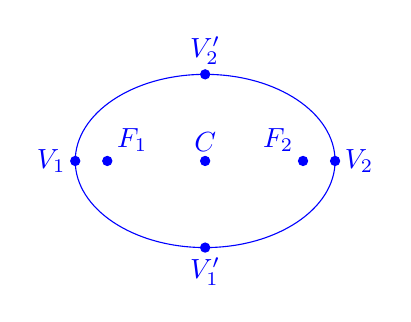
\begin{tikzpicture}[xscale=0.55,yscale=0.55]
        \draw[blue] (0,0) ellipse (3 and 2);
        \filldraw[blue] (0,0) circle (3pt) node[above] {$C$};
        \filldraw[blue] (3,0) circle (3pt) node[right] {$V_2$};
        \filldraw[blue] (-3,0) circle (3pt) node[left] {$V_1$};
        \filldraw[blue] (0,-2) circle (3pt) node[below] {$V_1'$};
        \filldraw[blue] (0,2) circle (3pt) node[above] {$V_2'$};
        \filldraw[blue] (2.26,0) circle (3pt) node[above left] {$F_2$};
        \filldraw[blue] (-2.26,0) circle (3pt) node[above right] {$F_1$};
    \end{tikzpicture}
\end{wrapfigure}   

\noindent are tall (like the one seen to the right).     

Let's break this equation down.  $(h,k)$ is the center of the ellipse.  $a$ is called the semi-major axis, or half the width of the ellipse.  The points at $ (h \pm a, k) $ are called the vertices.  $b$ is called the semi-minor axis, or half the height of the ellipse.  The points at $ (h,k \pm b) $ are called the co-vertices.  See the diagram to the right for a more visual explanation.

Lastly, we must introduce the foci (focus when singular).  Ellipses are defined as the set of all points where the sum of the distances to the two foci is constant.  The foci for horizontal

\begin{wrapfigure}{r}{5cm}
    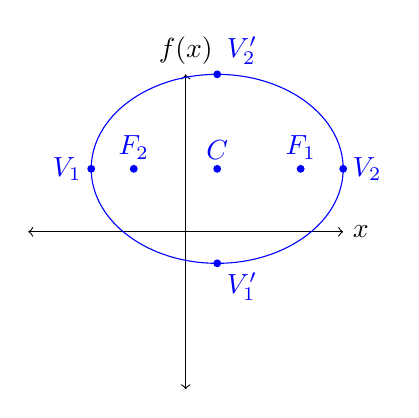
\begin{tikzpicture}[xscale=0.40,yscale=0.40]
        \draw[<->] (-5,0) -- (5,0) node[right] {$x$};
        \draw[<->] (0,-5) -- (0,5) node[above] {$f(x)$};
        \draw[blue] (1,2) ellipse (4 and 3); 
        \filldraw[blue] (1,2) circle (3pt) node[above] {$C$};
        \filldraw[blue] (5,2) circle (3pt) node[right] {$V_2$};
        \filldraw[blue] (-3,2) circle (3pt) node[left] {$V_1$};
        \filldraw[blue] (1,5) circle (3pt) node[above right] {$V_2'$};
        \filldraw[blue] (1,-1) circle (3pt) node[below right] {$V_1'$};
        \filldraw[blue] (-1.65,2) circle (3pt) node[above] {$F_2$};
        \filldraw[blue] (3.65,2) circle (3pt) node[above] {$F_1$};
    \end{tikzpicture}
\end{wrapfigure}

\noindent ellipses are located at $(h \pm c,k)$.  $c$ is a value called the focal radius, calculated using $c=\sqrt{a^2-b^2}$.  The foci are labeled in the graph to the right.

\begin{example}
Graph the equation $\frac{(x-1)^2}{16} + \frac{(y-2)^2}{9} = 1$.  Be sure to label the center, vertices, co-vertices, and foci.
\end{example}
\begin{solution}
See the graph below.
It should be clear from the equation that the center is $(1,2)$.  Looking at the two divisors, $16$ and $9$.  $a$ must be $\sqrt{16}=4$ because it is the larger divisor.  Hence, $b$ must be $\sqrt{9}=3$.  Remember the vertices are at $(h\pm a,k)$ for horizontal ellipses, so the vertices here are $(1 \pm 4,2)$.  The co-vertices are at $(h, k \pm b)$, so the co-vertices here are $(1,2 \pm 3)$.  Lastly, we can calculate that the focal radius is $c=\sqrt{a^2-b^2}=\sqrt{7}$.  The foci are at $(h \pm c ,k)$, so the foci here are at $(1 \pm \sqrt7, 2)$.  The graph is to the right of this solution at the bottom of the previous page. $\Box$
\end{solution}

\subsection{General Equation for (Vertical) Ellipses}

\begin{wrapfigure}{r}{5cm}
    \begin{tikzpicture}[xscale=0.20,yscale=0.20]
        \draw[<->] (-10,0) -- (10,0) node[right] {$x$};
        \draw[<->] (0,-10) -- (0,10) node[above] {$f(x)$};
        \draw[blue] (0,0) ellipse (7 and 4); 
    \end{tikzpicture}
\end{wrapfigure}

\noindent Now let's explore the general equation for "vertical" ellipses, those that are taller than they are wide.
$$ \frac{(y-k)^2}{a^2} + \frac{(x-h)^2}{b^2} = 1$$$$(a,b)\in\mathbb{R},a\neq 0,b\neq 0,a>b.$$

\noindent Notice, the only difference is that the $y$ part is now over $a^2$ while the $x$ part is now over $b^2$.  Because the ellipse is now 

\noindent taller, its vertices are at $(h,k \pm a)$ and its co-vertices are at

\noindent $(h \pm b, k)$.  Its foci are instead at $ (h,k \pm c) $.  Everything else remains the same.  See the diagram to the right for a visual explanation.

\begin{example}
Graph the equation $\frac{(y-3)^2}{36} + \frac{(x-2)^2}{4} = 1$.  Be sure to label the center, vertices, co-vertices, and foci.
\end{example}
\begin{solution}
It should be clear from the equation that the center is $(2,3)$.  Looking at the two
\end{solution}

\begin{wrapfigure}{r}{5cm}
    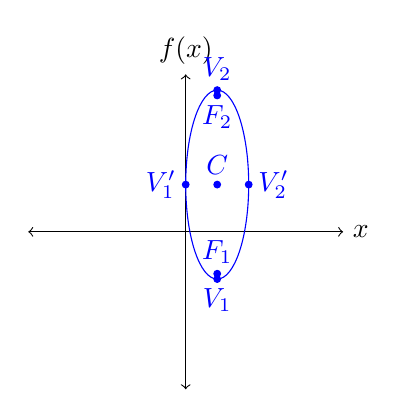
\begin{tikzpicture}[xscale=0.20,yscale=0.20]
        \draw[<->] (-10,0) -- (10,0) node[right] {$x$};
        \draw[<->] (0,-10) -- (0,10) node[above] {$f(x)$};
        \draw[blue] (2,3) ellipse (2 and 6); 
        \filldraw[blue] (2,3) circle (6pt) node[above] {$C$};
        \filldraw[blue] (2,9) circle (6pt) node[above] {$V_2$};
        \filldraw[blue] (2,-3) circle (6pt) node[below] {$V_1$};
        \filldraw[blue] (4,3) circle (6pt) node[right] {$V_2'$};
        \filldraw[blue] (0,3) circle (6pt) node[left] {$V_1'$};
        \filldraw[blue] (2,8.66) circle (6pt) node[below] {$F_2$};
        \filldraw[blue] (2,-2.66) circle (6pt) node[above] {$F_1$};
    \end{tikzpicture}
\end{wrapfigure}

\noindent divisors, $36$ and $4$.  $a$ must be $\sqrt{36}=6$ because it is the larger divisor.  Hence, $b$ must be $\sqrt{4}=2$.  Remember the vertices are at $(h,k \pm a)$ for vertical ellipses, so the vertices here are $(2,3 \pm 6)$.  The co-vertices are at $(h \pm b, k)$, so the co-vertices here are $(2 \pm 2,3)$.  Lastly, we can calculate that the focal radius is $c=\sqrt{a^2-b^2}=\sqrt{32} = 4\sqrt2$.  The foci are at $(h,k \pm c)$, so the foci here are at $(2,3\pm 4\sqrt2)$.  The graph is depicted to the right and uses the key below. $\Box$
$$\begin{matrix} C=(2,3) & V_1=(2,-3) & V_2=(2,9) \\ V_1'=(0,3) & V_2'=(4,3) & F_1=(2,3-4\sqrt{2}) \\ F_1=(2,3-4\sqrt{2}) & F_2=(2,3+4\sqrt{2}) \end{matrix}.$$

\subsection{Application: Kepler's First Law of Planetary Motion}
\noindent Kepler's First Law of Planetary Motion states that planets move in an elliptical orbit with the Sun at one of the two foci.

\begin{example}
At its closest point (perihelion), Mars is $1.4$AU from the Sun.  At its farthest point (aphelion), Mars is $1.7$AU from the Sun.  Use this information to find an equation for Mars's elliptical orbit.
\end{example}
\begin{solution}
Assume the center of the ellipse is at the origin.  Adding the two extreme distances will give us the value of the major axis $1.4+1.7=3.1$AU.  Therefore the semi-major axis $a= 3.1/2 = 1.55$AU.  

Furthermore, if the center is at the origin, then the Sun must be $1.7-1.4=0.3$AU offset from the center.  We can also call this distance the focal radius, so $c=0.3$AU.  

With $a$ and $c$, we can calculate $b$:
$$ c = \sqrt{a^2-b^2} \implies b = \sqrt{a^2-c^2} $$
Hence, $b = \sqrt{1.55^2-0.3^2} = \sqrt{1.25} \approx 1.1$AU.  

Let's plug these values into our general equation for a horizontal ellipse at the origin:
$$ \frac{x^2}{a^2} + \frac{y^2}{b^2} = 1 $$
This becomes
$$ \frac{x^2}{1.55^2} + \frac{y^2}{1.1^2} = 1 \implies \frac{x^2}{2.4} + \frac{y^2}{1.2} = 1.$$ $\Box$
\end{solution}
With this, we conclude our study of ellipses.  Hopefully, this wasn't terribly difficult, for it is only an extension of circles.  Finally, we will be studying parabolas $-$ a slight twist on the ellipse function to yield a completely new concept.
\section{Hyperbolas}
\noindent In this section, we introduce the final conic: hyperbolas.  As you will see in this section, hyperbolas resemble two opposite facing parabolas. Below are a depiction of a horizontal and a vertical hyperbola.

\begin{figure}[!h]
    \centering
    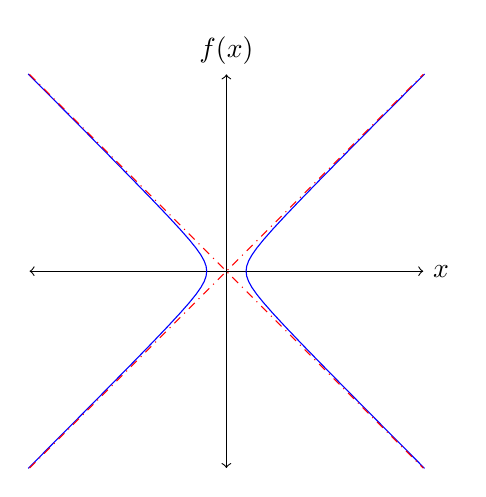
\begin{tikzpicture}[xscale=0.25,yscale=0.25]
        \draw[<->] (-10,0) -- (10,0) node[right] {$x$};
        \draw[<->] (0,-10) -- (0,10) node[above] {$f(x)$};
        \draw[scale=1,domain=-3:3,variable=\x,blue] plot ({cosh(\x)},{sinh(\x)});
        \draw[scale=1,domain=-3:3,variable=\x,blue] plot ({-cosh(\x)},{sinh(\x)});
        \draw[dashdotted,red,domain=-10:10,variable=\x] plot ({\x},{-\x});
        \draw[dashdotted,red,domain=-10:10,variable=\x] plot ({\x},{\x});
    \end{tikzpicture}
    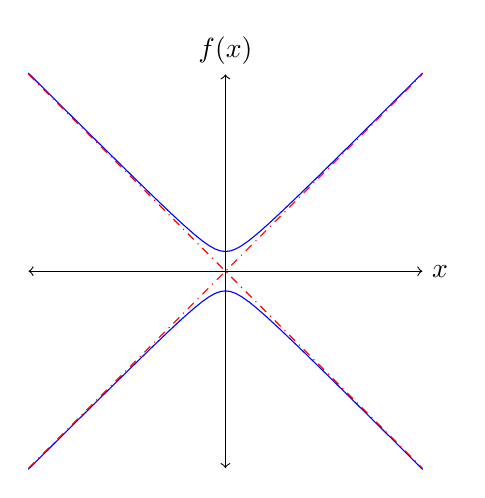
\begin{tikzpicture}[xscale=0.25,yscale=0.25]
        \draw[<->] (-10,0) -- (10,0) node[right] {$x$};
        \draw[<->] (0,-10) -- (0,10) node[above] {$f(x)$};
        \draw[scale=1,domain=-3:3,variable=\x,blue] plot ({sinh(\x)},{cosh(\x)});
        \draw[scale=1,domain=-3:3,variable=\x,blue] plot ({sinh(\x)},{-cosh(\x)});
        \draw[dashdotted,red,domain=-10:10,variable=\x] plot ({\x},{-\x});
        \draw[dashdotted,red,domain=-10:10,variable=\x] plot ({\x},{\x});
    \end{tikzpicture}
\end{figure}

Let's explore each type separately.
\subsection{General Equation for (Horizontal) Hyperbolas}
\noindent "Horizontal" hyperbolas open to the left and right and have a general equation of:
$$ \frac{(x-h)^2}{a^2} - \frac{(y-k)^2}{b^2} = 1; \hspace{5mm} (a,b)\in\mathbb{R},a\neq 0,b\neq 0,a<b.$$

Hopefully you can guess by now that $(h,k)$ is the center.  $a$ is the semi-major axis, or half the distance between the two "parabolas".  The points $(h \pm a,k)$ are called the vertices.  $b$ is the semi-minor axis.  The points $(h,k \pm b)$ are called the co-vertices.

Hyperbolas have a focal radius $c=\sqrt{a^2+b^2}$.  Notice that this is not the same calculation for ellipses (where $c=\sqrt{a^2-b^2}$).  The points $(h \pm c,k)$ are called the foci of the hyperbola.

\begin{wrapfigure}{r}{5cm}
    \begin{tikzpicture}[xscale=0.25,yscale=0.25]
        \draw[<->] (-10,0) -- (10,0) node[right] {$x$};
        \draw[<->] (0,-10) -- (0,10) node[above] {$f(x)$};
        \draw[scale=1,domain=-1.5:1.5,variable=\x,blue] plot ({4*cosh(\x)+1},{3*sinh(\x)});
        \draw[scale=1,domain=-1.5:1.5,variable=\x,blue] plot ({-4*cosh(\x)+1},{3*sinh(\x)});
        \draw[dashdotted,red,domain=-10:9,variable=\x] plot ({\x+1},{-0.75*\x});
        \draw[dashdotted,red,domain=-10:9,variable=\x] plot ({\x+1},{0.75*\x});
        \filldraw[red] (1,0) circle (3pt) node[above=3mm] {$(1,0)$};
        \filldraw[blue] (6,0) circle (3pt);
        \filldraw[blue] (-4,0) circle (3pt);
        \filldraw[blue] (5,0) circle (3pt) node[above right=0mm and 1mm] {$(5,0)$};
        \filldraw[blue] (-3,0) circle (3pt) node[above left=0mm and 1mm] {$(-2,0)$};
    \end{tikzpicture}
\end{wrapfigure}

The asymptotes are opposite in sign and the slope is the ratio of $b$ to $a$.  The formula for them are $y-k=\pm\dfrac{b}{a}(x-h)$.

Let's do an example.
\begin{example}
Graph the hyperbola $\frac{(x-1)^2}{16} - \frac{y^2}{9} = 1$.  Be sure to label the center, vertices, co-vertices, and foci.
\end{example}
\begin{solution}
The center is at $(1,0)$.  $16$ is the larger divisor, so $a=\sqrt{16}=4$.  Therefore, $b=\sqrt{9}=3$.  We can calculate the focal radius $c=\sqrt{16+9}=5$.  The vertices are at $(h \pm a ,k) = (1 \pm 4,0)$.  The co-vertices are at $(h,k \pm b)=(1,\pm 3)$.  The foci are at $(h \pm c,k) = (1 \pm 5, 0)$.  The asymptotes are thus $y-0=\pm\dfrac{3}{4}(x-1) \implies y=\pm\dfrac{3}{4}(x-1)$.  See the graph to the right $-$ unfortunately, due to space limitations, there wasn't space to label the co-vertices and the foci. $\Box$
\end{solution}

\subsection{General Equation for (Vertical) Hyperbolas}
\noindent Just like the other conics, hyperbolas can also be oriented vertically.  The general equation for 

\begin{wrapfigure}{r}{5cm}
    \begin{tikzpicture}[xscale=0.05,yscale=0.05]
        \draw[<->] (-50,0) -- (50,0) node[right] {$x$};
        \draw[<->] (0,-50) -- (0,50) node[above] {$f(x)$};
        \draw[scale=1,domain=-2:2,variable=\x,blue] plot ({5*sinh(\x)},{12*cosh(\x)});
        \draw[scale=1,domain=-2:2,variable=\x,blue] plot ({5*sinh(\x)},{-12*cosh(\x)});
        \draw[dashdotted,red,domain=-20.8:20.8,variable=\x] plot ({\x},{-2.4*\x});
        \draw[dashdotted,red,domain=-20.8:20.8,variable=\x] plot ({\x},{2.4*\x});
    \end{tikzpicture}
\end{wrapfigure}

\noindent vertical hyperbolas is:
$$ \frac{(y-k)^2}{b^2} - \frac{(x-h)^2}{a^2} = 1$$$$(a,b)\in\mathbb{R},a\neq 0,b\neq 0,a<b.$$

Many properties from horizontal hyperbolas carry over.  $(h,k)$ is the center, $a$ is the semi-major axis, $b$ is the semi-minor axis, and $c=\sqrt{a^2+b^2}$ is the focal radius.  However, $(h,k \pm a)$ are the vertices, $(h \pm b)$ are the co-vertices, and $(h,k \pm c)$ are the foci.

\begin{example}
Graph the hyperbola $\frac{y^2}{144} - \frac{x^2}{25} = 1$.  Be 

\noindent sure to label the center, vertices, co-vertices, and foci.
\end{example}

\begin{solution}
The center is at $(0,0)$.  $144$ is the larger divisor, so $a=\sqrt{144}=12$.  Therefore, $b=\sqrt{25}=5$.  We can calculate the focal radius $c=\sqrt{144+25}=13$.  The vertices are at 
\end{solution}

\noindent $(h, k \pm a) = (0,\pm 12)$.  The co-vertices are at $(h\pm b,k)=(\pm 5,0)$.  The foci are at $(h ,k \pm c) = (0, \pm 13)$.  We use the formula for the asymptotes to see the asymptotes are at $y(x)=\pm\dfrac{12}{5}x.$ See the graph at the bottom of the previous page for the graph. $\Box$

\section{A Note on Rational Functions}
\begin{wrapfigure}{r}{5cm}
    \begin{tikzpicture}[xscale=0.25,yscale=0.25]
        \draw[<->] (-10,0) -- (10,0) node[right] {$x$};
        \draw[<->] (0,-10) -- (0,10) node[above] {$f(x)$};
        \draw[scale=1,domain=-10:-0.1,variable=\x,blue] plot ({\x},{1/\x});
        \draw[scale=1,domain=0.1:10,variable=\x,blue] plot ({\x},{1/\x});
    \end{tikzpicture}
\end{wrapfigure}

\noindent How many of the four conics can be represented by functions (passing the vertical line test)?  The seemingly obvious answer is one, just parabolas because they can be represented by functions like $y=x^2$ when they are vertically oriented.  However, we've failed to mention up to this point that conics are not just oriented horizontally or vertically.  Instead, they can be rotated by any angle and still be considered a conic.  Consider a rotation of the hyperbola given by $x^2-y^2=1$ by an angle of $45^{\circ}$ or $\frac{\pi}{4}$ radians.  This results in the graph seen below.

Maybe you will recognize this as the function $y=\frac{1}{x}$ or $xy=1$.  This equation satisfies the vertical line test and represents a hyperbola.  Therefore, there are two conics that can be represented by functions: (vertically-oriented) parabolas and (diagonally-oriented) hyperbolas.

Proving this is a bit beyond the scope of this book, but if you can prove it, you'll be well on your way to succeeding at Pre-calculus.  Here's a hint: the formal definition of a hyperbola is a set of points where the positive difference between $dist(P-F_1)$ and $dist(P-F_2)$ for arbitrary point $P$ is the same. This task will be in the challenge problems.

With this, we conclude the discussion of Conics.  This was not an easy chapter, but learning it now will make studying it in the Spring a lot easier.  Proceed to the Review and Challenge problems and attempt to do them, but don't worry if you can't solve them all.  
\begin{reviewset}
\item Find the vertex and axis of symmetry of the following equations, then graph them. \newline 
(a) $y=4x^2-12x+8$. \hspace{\stretch{1}} (b) $x=\dfrac{1}{6}(y-4)^2-1$ \hspace{\stretch{1}} \vspace{3mm}
\item The vertex of the parabola $x=4y^2+6y+c$ lies on the $y$-axis.  Find $c$. \vspace{3mm}
\item For each of the two descriptions below, find an equation to represent the function. \newline 
(a) An ellipse with vertices at $(3,6)$ and $(3,-2)$ and co-vertices at $(0,2)$ and $(6,2)$. \newline
(b) A hyperbola with vertices at $(-2,1)$ and $(-2,3)$ with asymptotes sloped at $\pm\dfrac{1}{2}$. \newline
(c) A parabola with vertex $(2,1)$ and $y$-intercept of $(0,3)$. \vspace{3mm}
\item Find the indicated value for the following functions. \newline 
(a) The minimum of $x(y)=2y^2-4y+19$. \newline 
(b) The maximum of $y(x)=37-16x-x^2$. \newline 
(c) The minimum of $x^2+4y^2-6x+4y+5$. \vspace{3mm}
\item Find the area enclosed in the graph $x^2+y^2=16x+32y$. (Hint: consider how we find the area of a circle.  Try re-writing the formula in terms of the axes lengths so it's applicable to an ellipse). \vspace{3mm}
\item Graph each of the equations below, then find the foci, center, and lengths of the axes of each graph. \newline 
(a) $\dfrac{(x-3)^2}{9}+y^2=1$ \hspace{\stretch{1}} (b) $4x^2+y^2+16x-6y=11$ \hspace{\stretch{1}} \vspace{3mm}
\item Ellipse $\mathcal{E}$ has a horizontal major axis, one focus at $(4,1)$, and one axis with an endpoint at $(6,5)$.  Find an equation whose graph is this ellipse. \vspace{3mm}
\item Find the center, asymptotes, and vertices of the graphs of each equation below, then graph each equation. \newline
(a) $x^2-4(y+1)^2=1$ \hspace{\stretch{1}} (b) $2x^2-y^2+8x+6y=9$  \hspace{\stretch{1}} \vspace{3mm}
\end{reviewset}
\begin{challengeset}
\item An airline company currently charges $\$200$ per ticket, and sells $40,000$ tickets. For every $\$10$ they increase the ticket prise, they sell $1000$ fewer tickets. How much should they charge to maximize their revenue? (Hint: make an equation $-$ it should be a conic!) \vspace{3mm}
\item One of the graphs of the following equations comes within $1$ unit of the point $(265,346)$. Which one? \newline 
(A) $y^2+x+4y+7=0$ \hspace{\stretch{1}} (B) $x^2+y^2+4y+17=0$ \hspace{\stretch{1}} \newline
(C) $16x^2-96x-9y^2-54y=81$ \hspace{\stretch{1}} (D) $25x^2+9y^2-36y=9$ \hspace{\stretch{2}} \vspace{3mm}
\item Prove that $y(x)=\dfrac{1}{x}$ is a hyperbola; find the foci of the function. \vspace{3mm}
\item The \textit{latus rectum} of an ellipse is a line segment with both endpoints on the ellipse that is parallel to the minor axis and passes through the focus of the ellipse.  Find the length of a latus rectum of the graph of $\dfrac{x^2}{a^2}+\dfrac{y^2}{b^2}=1$ in terms of $a$ and $b$. \vspace{3mm}
\item If $x$ is real, then determine the maximum value of $\dfrac{3x^2+9x+17}{3x^2+9x+7}$. \vspace{3mm}
\item Given that $x^2+y^2=14x+6y+6$, what is the largest possible value that $3x+4y$ can have? (There's a cool calculus way to do this, but stick with the geometry/algebra way.)\vspace{3mm}
\end{challengeset}
\end{document}